%%%%%%%%%%%%%%%%%%%%%%%%%%%%%%%%%%%%%%%%%%%%%%%%%%%%%%%%%%%%%%%%%%%%%%%%

%%% LaTeX Template for AAMAS-2023 (based on sample-sigconf.tex)
%%% Prepared by the AAMAS-2023 Program Chairs based on the version from AAMAS-2022. 

%%%%%%%%%%%%%%%%%%%%%%%%%%%%%%%%%%%%%%%%%%%%%%%%%%%%%%%%%%%%%%%%%%%%%%%%

%%% Start your document with the \documentclass command.
%%% Use the first variant below for the final paper.
%%% Use the second variant below for submission.

\documentclass[sigconf]{aamas} 
% \documentclass[sigconf,anonymous]{aamas} 

%%% Load required packages here (note that many are included already).

\usepackage{balance} % for balancing columns on the final page
\usepackage{tikz}
\newcommand{\drawNaivePricingFigure}{
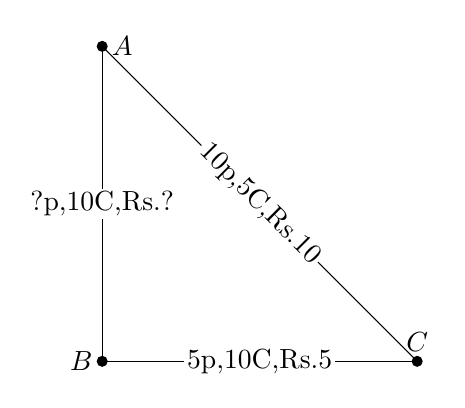
\begin{tikzpicture}
    % Define coordinates for the three nodes A, B, and C
    \coordinate (A) at (0, 4);
    \coordinate (B) at (0, 0);
    \coordinate (C) at (4, 0);

    % Draw the edges and label them using the 'midway' option
    % Edge A -- B
    \draw (A) -- (B) node [midway, fill=white, inner sep=1pt] {?p,10C,Rs.?};

    % Edge A -- C
    \draw (A) -- (C) node [midway, fill=white, inner sep=1pt, sloped] {10p,5C,Rs.10};

    % Edge B -- C
    \draw (B) -- (C) node [midway, fill=white, inner sep=1pt, sloped] {5p,10C,Rs.5};

    % Draw and label the vertices (Nodes)
    \fill (A) circle (2pt) node [right] {$A$};
    \fill (B) circle (2pt) node [left] {$B$};
    \fill (C) circle (2pt) node [above] {$C$};

\end{tikzpicture}
}
%%%%%%%%%%%%%%%%%%%%%%%%%%%%%%%%%%%%%%%%%%%%%%%%%%%%%%%%%%%%%%%%%%%%%%%%

%%% AAMAS-2023 copyright block (do not change!)

\setcopyright{ifaamas}
\acmConference[AAMAS '26]{Proc.\@ of the 25th International Conference
on Autonomous Agents and Multiagent Systems (AAMAS 2026)}{May 29 -- June 2, 2026}
{London, United Kingdom}{A.~Ricci, W.~Yeoh, N.~Agmon, B.~An (eds.)}
\copyrightyear{2025}
\acmYear{2025}
\acmDOI{}
\acmPrice{}
\acmISBN{}

%%%%%%%%%%%%%%%%%%%%%%%%%%%%%%%%%%%%%%%%%%%%%%%%%%%%%%%%%%%%%%%%%%%%%%%%

%%% Use this command to specify your EasyChair submission number.
%%% In anonymous mode, it will be printed on the first page.

\acmSubmissionID{???}

%%% Use this command to specify the title of your paper.

\title[Pricing New Routes]{Pricing of Upcoming Routes in a Capacity Constrained Transport Network: Kolkata Metro}

%%% Provide names, affiliations, and email addresses for all authors.

\author{Arghya }
\affiliation{
  \institution{IITB}
  \city{Mumbai}
  \country{India}}
% \email{king.arthur@camelot.uk}

\author{Sagar }
\affiliation{
  \institution{IITB}
  \city{Mumbai}
  \country{India}}

\author{Shivang }
\affiliation{
  \institution{IITB}
  \city{Mumbai}
  \country{India}}

\author{Abhishek}
\affiliation{
  \institution{IITB}
  \city{Mumbai}
  \country{India}}
%%% Use this environment to specify a short abstract for your paper.

\begin{abstract}
Rapid urbanisation has led to increased investments by governments in developing rapid transit systems like metros to decrease strain on existing transport networks of a city. However, naively setting prices for these new routes can lead to congestion as they enable alternate routes to the commuters to reach their destinations. In this work, we study how to set prices for upcoming routes while also staying within the capacity constraints. We aim to build tools that help decision makers set prices in a manner that balances the various tradeoffs involved.

Game theory allows us to reason about traffic load distribution at equilibrium. We used Wardrop's principles to build a tool for setting prices for upcoming routes in a general transport network. We ran experiments on a model of Kolkata metro - one of the oldest rapid transit systems in the country - to suggest prices for its upcoming extensions. We show how the capacity constraints are respected and also discuss how our tool can be extended to balance other tradeoffs such as maximizing revenue and improving social welfare.

\end{abstract}

%%% The code below was generated by the tool at http://dl.acm.org/ccs.cfm.
%%% Please replace this example with code appropriate for your own paper.


%%% Use this command to specify a few keywords describing your work.
%%% Keywords should be separated by commas.

\keywords{Game Theory, Transportation Networks, Dynamic Pricing}

%%%%%%%%%%%%%%%%%%%%%%%%%%%%%%%%%%%%%%%%%%%%%%%%%%%%%%%%%%%%%%%%%%%%%%%%

%%% Include any author-defined commands here.
         
\newcommand{\BibTeX}{\rm B\kern-.05em{\sc i\kern-.025em b}\kern-.08em\TeX}

%%%%%%%%%%%%%%%%%%%%%%%%%%%%%%%%%%%%%%%%%%%%%%%%%%%%%%%%%%%%%%%%%%%%%%%%

\begin{document}

%%% The following commands remove the headers in your paper. For final 
%%% papers, these will be inserted during the pagination process.

\pagestyle{fancy}
\fancyhead{}

%%% The next command prints the information defined in the preamble.

\maketitle 

%%%%%%%%%%%%%%%%%%%%%%%%%%%%%%%%%%%%%%%%%%%%%%%%%%%%%%%%%%%%%%%%%%%%%%%%

\section{Introduction}
\label{sec:intro}

Transportation networks have become an essential part of urban planning. The ability to rapidly move large numbers of commuters from residential to industrial or tourist parts of a city is critical for its economic growth.
As road congestion and traffic problems continue to worsen, governments across the world are investing aggresively towards expanding rapid transit systems like metros. As new routes are added, commuters get access to alternate direct or indirect routes to reach their destinations.

\begin{figure}[h]
    \centering
    \drawNaivePricingFigure
    \caption{Ex: Setting Low prices can lead to exceding capacity}
    \label{fig:naivePricing}
\end{figure}

The two most crucial factors influencing a commuter's preferences between alternative routes are the total price of the route and the congestion on it. 
Consider three cities A, B and C connected via metro lines as shown in Figure \ref{fig:naivePricing}. If say \( 10 \) and $5$ be the number of commuter travelling daily from A to C and from B to C respectively, while the capacity of the routes are 5 each and the ticket prices are $10$ and $5$. Suppose a new metro line AB is opened with a capacity of $10$. If the route AB is priced less than $5$ then all $10$ commuters from A to C will prefer the route A-B-C leading to exceeding capacity on the route B-C. On the other hand if the price is set too high then none of the commuters will use the new route, wasting public resources. 
Hence a naive approach of pricing based on demand surveys between source-destination pairs without considering how the flow redistributes may lead to exceeding capacity or underutilisation on certain routes of the network.

Congestion is another factor that influences commuter preferences over the routes. Highly congested routes would be avoided by commuters even if they are cheaper. Although they might still prefer metro over buses (or newer metro over older) given same congestion and price incurred on both the routes. To capture this we model the cost incurred by a commuter on a route to be \(kx + p \) where \(k\) is the congestion factor of the route, \(x\) the number of commuters using the route and \(p\) is the price of using the route. Each commuter would then choose the route that incurrs them the least net cost. 

The prices must thus be set so that all routes operate within capacity and no resources are underutilised. Although the government may generate revenue, the economic activity enabled by the network far outweights the cost to maintainan them. Thus for social welfare the average cost incurred by commuters must also be kept low. 

Game theoretic ideas have been proposed as early as 1950s by Wardrop \cite[p. 344]{wardrop_road_1952} to study distribtuion of traffic flows between alternative routes of a network. Wardrop's principle can be stated as follows:

At equillibrium, the cost incurred by all used routes between a source-destination pair is equal and less than the cost that would be incurred by using any unused route. Thus a new commuter should be indifferent between all used routes.
Using this principle we model the problem of setting prices for new routes as a constraint optimisation problem. The constraints being to operate within capacity and the objective function being to maximise the social welfare of the commuters.

We chose Kolkata metro network for our experiments. Kolkata metro is one of the oldest metro system in India with multiple extensions planned in the near future. It also caters to both rich and poor stratas of the society covering 
most parts of the city. This gives us a good oppurtunity to predict the impact of pricing on congestion, the average cost incurred by the commuters and the revenue generated by the government. We also study the impact of the order in 
which the new routes are added.

While the focus of the current work is on maximising social welfare, we also suggest how our tool can be extended for other considerations. Sometimes generating a minimum revenue is required to cover operating costs. Not all neighbourhoods are equally sensitive to prices, and ensuring fairness in pricing for poorer commuters is important.
Parking constraints in certain localities may also lead to governments incentivising prices for some routes to promote metro usage. We leave these for future work. 

The rest of the report is organised as follows. In Section \ref{sec:related} we look at some of the previous works 
on pricing of transport networks. In Section \ref{sec:kolkataMetro} we track the development of Kolkata metro to its current state. In Section \ref{sec:Model} we describe our mathematical model for pricing new routes. In Section \ref{sec:ExpResults} we report the experiments conducted and the results obtained. Finally in Section \ref{sec:Conclusion} we conclude with a summary and future work.
%%%%%%%%%%%%%%%%%%%%%%%%%%%%%%%%%%%%%%%%%%%%%%%%%%%%%%%%%%%%%%%%%%%%%%%%
\subsection{Related Work}
\label{sec:related}

TODO: In this section, we discuss some of the previous works related to pricing transportation routes and managing congestion in urban transportation networks and contrast them with our approach.

TODO: Traffic flow distribution when commuters can choose between alternative routes was studied as early as 1950's. \cite{wardrop_correspondence_1952,wardrop_road_1952} Came up with two principles -- solving for which gives the equilibrium conditions. -- our work closely relates to them although -- they studied road networks with cost incurred to a commuter being average time taken for a journey -- for us cost is congestion factor and ticket prices -- they study various interventions like road width, layout design, traffic control signals while we only consider setting prices for the new new route. \\
\cite{saharan_dynamic_2020} Do a survey of dynamic pricing in transport networks -- in most settings though the prices of a route can be set in real time based and changing demands -- we keep only set them once when a new route is opened up -- Other than game theory, queeing theory methods also discussed.
\cite{hintermann_beat_et_al_pigovian_2025} Work focusses on practical challenges on implementing pigovian strategies -- including pricing taxing etc.-- they measure system utility based on external factors like climate change /health congestion when passsnegers have choices between different modes of transportation -- unlike us they do consider choices betweeen alternate routes. \\
\cite{liu_research_2015} Again study the whole network pricing policy and not individual edges --  model it as three party game -- govenrnment, corporations,
and commuters each having different objectives. They also suggest different pricing for non- peak peak dmands and rural /urban neighbourhoods. We do consider them in our but address them in our future works section \\
\cite{mozafari_dynamic_2015} Study freight networks. The tradeoff again are not between alternative routes but setting prices so as to beat competitors for 
transporting goods. The pricing decided by the transport company have to also depend on the fleet availabiity which is dynamic but for in our model the capacity of a route do not change.  \\
\cite{zhang_optimal_2024} Again they do not study under the alternative routes but alternative modes of transport network between a source and destination.
-- The network they consider is the social netwrok by which consumer preferences of the differennt modes of transport gets transferrred. The operators must continuously cahnge rpices inorder to beat the other operators while also keeping its current commuters happy else their prefernce gets learned via the social netwrok. \\

In the next section we study Kolkata metro system -- role in it public transport system. 

\subsection{Kolkata Metro Network}
\label{sec:kolkataMetro}

\begin{figure}
    \centering
    \includegraphics[width=0.8\linewidth]{example-image}
    \caption{Kolkata Metro Map with Upcoming Extension}
    \label{fig:4}
\end{figure}

\begin{figure}
    \centering
    \includegraphics[width=0.8\linewidth]{example-image}
    \caption{Existing Fare Card}
    \label{fig:3}
\end{figure}

TODO: Exisitng lines -- Upcoming projects -- Utilities -- Existing Fares -- Current Demand -- Residential /Industrial Regions.  



%%%%%%%%%%%%%%%%%%%%%%%%%%%%%%%%%%%%%%%%%%%%%%%%%%%%%%%%%%%%%%%%%%%%%%%%

\section{Mathematical Model}
\label{sec:Model}

Let \( G:= (V,E) \)  be a multigraph representing the transportation network where \( V \) represent the Important hubs (Major Stations or Depots or Transfer Points) of the city and \(E \) denote if two hubs are connected via a direct metro/bus line. 
For each edge we also store the data, {e.data = ($k$,colour, capacity, price)}, where $k$ denotes the congestion factor, colour - the metro line colour (or bus route number) and price is the ticket price for the direct line. 

We also maintain a list of demands, \(\mathcal{D} = \{D_i\}_{i} \) where \( D_i = (s_i, t_i, d_i) \) denotes that there are \( d_i \) commuters wishing to travel from source \( s_i \) to destination \( t_i \). 
 
When a new line is added to the network, we find for each demand \(D_i\) a list of Routes available to it via G, \( \mathcal{R}_i = \{R_{ij} \}_{j} \) where each route \( R_{ij} \) is a list of edges connecting \( s_i \) to \( t_i \). Let \( f_{R} \) be the number of commuters choosing route \( R \). Let \(f_e \) be the net flow on edge $e$. We have the following constraints:

\begin{gather}
  \sum_{\substack{R \in \cup \mathcal{R}_i, \\ e \in R}} f_{R} = f_e \quad \forall e \in E  \tag{C1} \\
  f_e \leq e.capacity \quad \forall e \in E  \tag{C2} \\
  \sum_{R \in \mathcal{R}_i} f_{R} = d_i \quad \forall D_i \in \mathcal{D}  \tag{C3} \\
  \intertext{If $f_R,f_{R'} \geq 0$, \(R, R' \in \mathcal{R}_i \) for some i then;}
  \sum_{e \in R} ((e.k)f_e + e.price ) = \sum_{e \in R'} ((e.k)f_e + e.price ) \tag{C4} \\
  \intertext{If $f_R \geq 0$ and $f_{R'} = 0$, \(R, R' \in \mathcal{R}_i \) for some i then;}
  \sum_{e \in R} ((e.k)f_e + e.price ) \leq \sum_{e \in R''} ((e.k)f_e + e.price ) \tag{C5}
\end{gather}

Here (C1) follows from the definition of flow on edges, (C2) ensures that no edge exceeds its capacity, (C3) ensures that all commuters are take some Route, (C4) and (C5) follow wardrop's principles that at equillibrium no commuter can reduce their cost by unilateral deviation.

To ensure social welfare, we set the objective to minimise the following function:
\begin{equation}
    F =  \sum_{D_i \in \mathcal{D}} \sum_{R \in \mathcal{R}_i} f_R \left( \sum_{e \in R} ((e.k)f_e + e.price ) \right)
\end{equation}
under the constraints (C1) - (C5). 
%%%%%%%%%%%%%%%%%%%%%%%%%%%%%%%%%%%%%%%%%%%%%%%%%%%%%%%%%%%%%%%%%%%%%%%%

\section{Experiments and Results}
\label{sec:ExpResults}

We used publicly available including Google Maps and Wikipedia to estimate the parameters needed to build our model of Kolkata Metro as described in Section \ref{sec:Model}. 
The demand for direct routes between hubs were set based on population density, availability of public utilities like airports, hospitals nearby and location of offices/industries. Each direct route was thus classified High / Medium / Low demand and the demands were set randomly within a range for each class so that the total demand nearly matched the reported daily ridership of Kolkata metro \cite{metro_railway_kolkata_metro_2025}.
$k$ was chosen to be 2 for all bus routes and less than 1 for metro lines depending on how old the line was. The capacity of each route was set based on current ridership on the line divided by the number of stations on the line, while for bus routes it was kept constant for all direct routes. We used exsiting fare charts to set the prices for the existing routes. 

Z3 solver \cite{z3_user_guide} was used to encode the constraints C1 - C5 and set a very high price for all new routes. We then used binary search to find the minimum price at which the constraints were satisfed. Z3 is a general purpose SMT solver and was able to check satisfyiablity of our constraints in reasonable time.
To limit the number of constraints, we pruned the max length of a route to be 4 hops. This is reasonable since since every transfer takes away valuable time of the commuters.
We also perform a sensitivity analysis by changing the parameters like demand, capacity and congestion factor by small amounts to see how they impact the results.
More details can be found in the code repository \ref{github}. 

Figure \ref{fig:1} shows traffic load at four transfer hubs i.e. sum of edge flows at the hub of the network before and after adding new routes. We can see that the capacity constraints are respected and the load decreases as more routes are added indicating better distribution of traffic flows.

Figure \ref{fig:2} shows the revenue generated by the government vs the average cost incurred by commuters as routes were added in different orders. We can see that the order in which routes are added did not have a significant impact on the average cost or Revenue generated.

Figure \ref{fig:3} shows a scatter plot of the revenue generated by the government vs the average cost incurred by commuters for different parameters settings. Changing parameters do not seem to have any major impact.


\begin{figure}
    \centering
    \includegraphics[width=0.8\linewidth]{example-image}
    \caption{Traffic Load at 4 Major Transfer Hubs: From left to right as more new routes are added to the network}
    \label{fig:1}
\end{figure}

\begin{figure}
    \centering
    \includegraphics[width=0.8\linewidth]{example-image}
    \caption{Revenue Generated/ Avg Cost time w.r.t order adding lines}
    \label{fig:2}
\end{figure}

\begin{figure}
    \centering
    \includegraphics[width=0.8\linewidth]{example-image}
    \caption{Revenue Generated/ Avg Cost time w.r.t changing parameters}
    \label{fig:3}
\end{figure}


%%%%%%%%%%%%%%%%%%%%%%%%%%%%%%%%%%%%%%%%%%%%%%%%%%%%%%%%%%%%%%%%%%%%%%%%
\section{Conclusion}
\label{sec:Conclusion}
TODO: Our Tool gives a principled approach for pricing new routes under Capacity Constraints -- We demonstrate its usability for pricing the
upcoming extensions on the kolkata metro network. -- we show how the average cost of a commuter can be reduced without losing a lot of revenue for the government while also not exceding the capacity constraints of the existing and new routes. -- Draw backs -- alongside bus networks/other means of transport 
-- Price sensitivity of commuters based on Neighbourhoods -- parking Availabilty in certain nodes -- We Show how these can be mitigated by simple cahnges to our approach.  

\subsection{Future Work}

TODO: Models parameters Objective Function that needs to be changed for addresing the above issues.

%%%%%%%%%%%%%%%%%%%%%%%%%%%%%%%%%%%%%%%%%%%%%%%%%%%%%%%%%%%%%%%%%%%%%%%%

%%% The following command should be issued somewhere in the first column 
%%% of the final page of your paper.
% \balance

%%%%%%%%%%%%%%%%%%%%%%%%%%%%%%%%%%%%%%%%%%%%%%%%%%%%%%%%%%%%%%%%%%%%%%%%

\section{References}


%%%%%%%%%%%%%%%%%%%%%%%%%%%%%%%%%%%%%%%%%%%%%%%%%%%%%%%%%%%%%%%%%%%%%%%%

%%% The acknowledgments section is defined using the "acks" environment
%%% (rather than an unnumbered section). The use of this environment 
%%% ensures the proper identification of the section in the article 
%%% metadata as well as the consistent spelling of the heading.

\begin{acks}
% Deeksha and Prof. 
\end{acks}

%%%%%%%%%%%%%%%%%%%%%%%%%%%%%%%%%%%%%%%%%%%%%%%%%%%%%%%%%%%%%%%%%%%%%%%%

%%% The next two lines define, first, the bibliography style to be 
%%% applied, and, second, the bibliography file to be used.

\bibliographystyle{ACM-Reference-Format} 
\bibliography{dynamicPricing.bib}

%%%%%%%%%%%%%%%%%%%%%%%%%%%%%%%%%%%%%%%%%%%%%%%%%%%%%%%%%%%%%%%%%%%%%%%%

\end{document}

%%%%%%%%%%%%%%%%%%%%%%%%%%%%%%%%%%%%%%%%%%%%%%%%%%%%%%%%%%%%%%%%%%%%%%%%

